\chapter{Visualisation}

\section{Introduction}
Pour la visualisation géographique des données, nous avons utilisé les technologies suivantes~:
\begin{itemize}
    \item Python~;
    \item Flask (serveur web)~;
    \item Scikit-learn (librairie de data mining)~;
    \item Google Maps API.\\
\end{itemize}

Avant de commencer toute tentative de représentation des données sous forme de cluster, nous avons commencé par afficher les points sur la carte.
Étant donné qu'il y environ 80~000 points, nous ne pouvons en afficher qu'une partie, en raison de la lenteur observée sur les navigateurs lors du rendu de la carte.

Nous avons opté pour le rendu d'un pourcent des points. La figure \vref{fig:points} présente le rendu d'un échantillon des points.

\begin{figure}[!h]
    \centering
    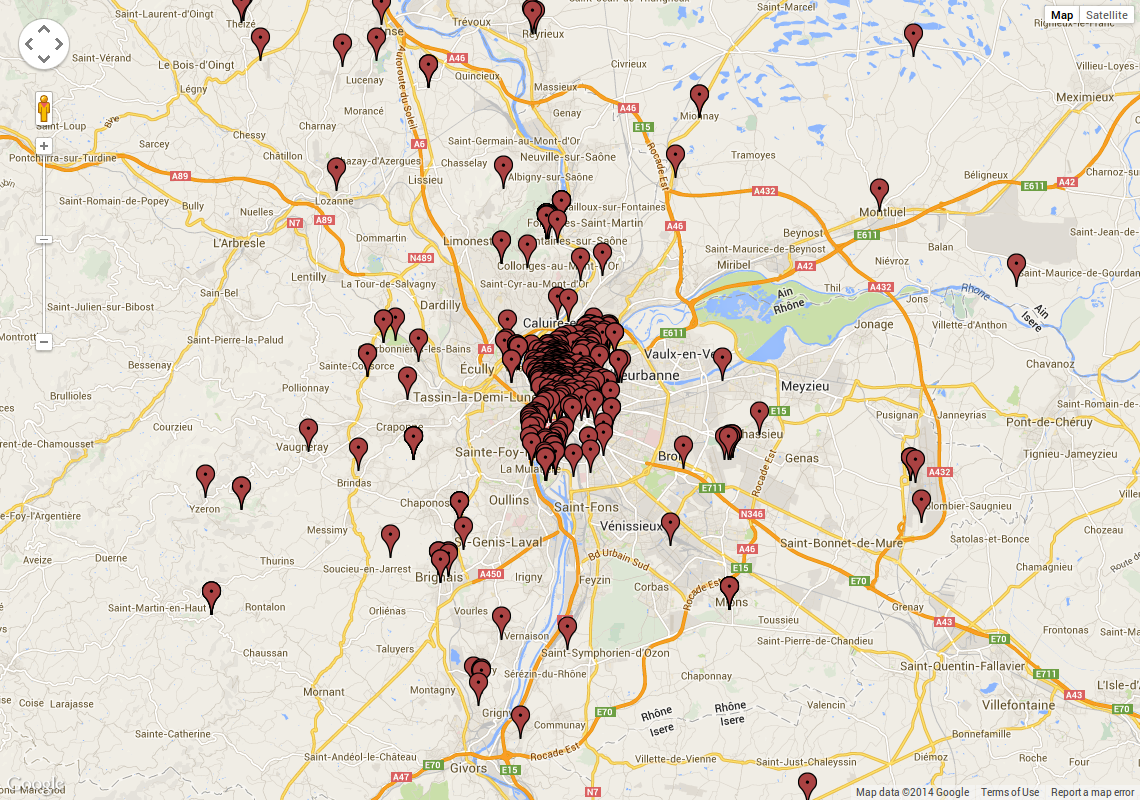
\includegraphics[width=14cm]{images/points.png}
    \caption{Affichage d'un échantillon des points}
    \label{fig:points}
\end{figure}

Cela nous donne déjà un premier aperçu. Nos points sont répartis autour de la ville de Lyon, et on constate une forte densité de points dans la ville.

Mais zoomons entre les deux fleuves de Lyon (figure \vref{fig:imprecision}).

\begin{figure}[!h]
    \centering
    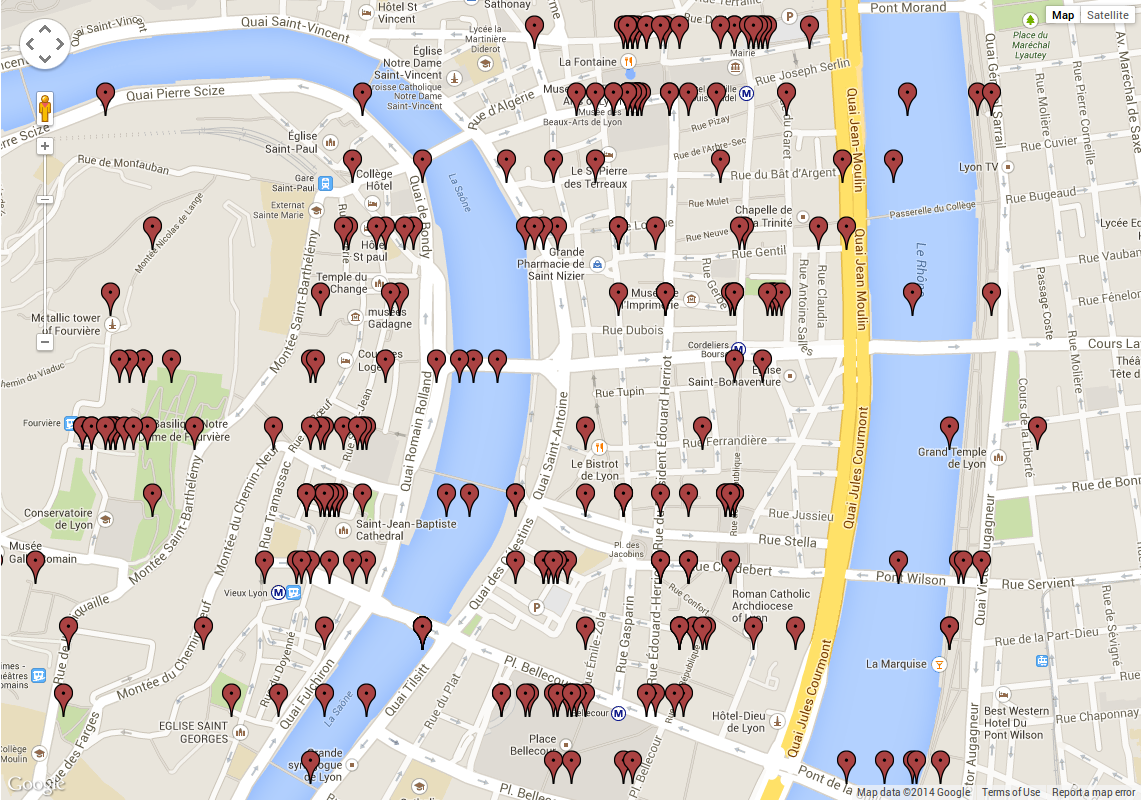
\includegraphics[width=14cm]{images/imprecision.png}
    \caption{Imprécision détectée lors du zoom}
    \label{fig:imprecision}
\end{figure}

On constate que tous les points se trouvent sur des lignes dont la séparation est très nette. Cela est dû à un manque de précision dans nos données de départ. Dans le fichier CSV initial, nous remarquons en effet que les coordonnées GPS les plus précises que nous avons ne comportent que 4 chiffres après la virgule, ce qui explique la répartition étrange des points sur des lignes. Nous savons donc que cette erreur aura un impact sur la qualité de nos futurs clusters.


\section{Meanshift}
Nous avons choisi d'appliquer l'algorithme de clustering \textbf{Meanshift}, pour tenter de trouver des clusters géographiques intéressants.

De manière très haut niveau, l'algorithme de clustering Meanshift peut être résumé comme suit~:
\begin{itemize}
    \item fixer une fenêtre autour de chaque point~;
    \item calculer la moyenne (le barycentre) des points à l'intérieur de cette fenêtre~;
    \item déplacer (\textit{shift}) la fenêtre sur la moyenne (\textit{mean}) et répéter ces étapes jusqu'à atteindre une convergence.\\
\end{itemize}

Nous avons choisi de représenter les clusters par des cercles dont l'aire est proportionnelle au nombre de points contenus dans le cluster. Chaque cercle est coloré aléatoirement, et son centre est le centre du cluster.
Le rayon du cercle en mètres est de~: $r = 10 \times \sqrt{n}$, où $n$ est le nombre de points présents dans le cluster. L'usage de la racine carrée nous permet d'éviter d'avoir une taille de cercle trop importante dans le cas de gros clusters.

La figure \vref{fig:meanshift1} montre le résultat d'un premier lancement de l'algorithme Meanshift avec un quantile de $0.2$ et un nombre minimal de points par cluster de $15$. Nous n'avons pas affiché les points pour plus de clarté.

\begin{figure}[!h]
    \centering
    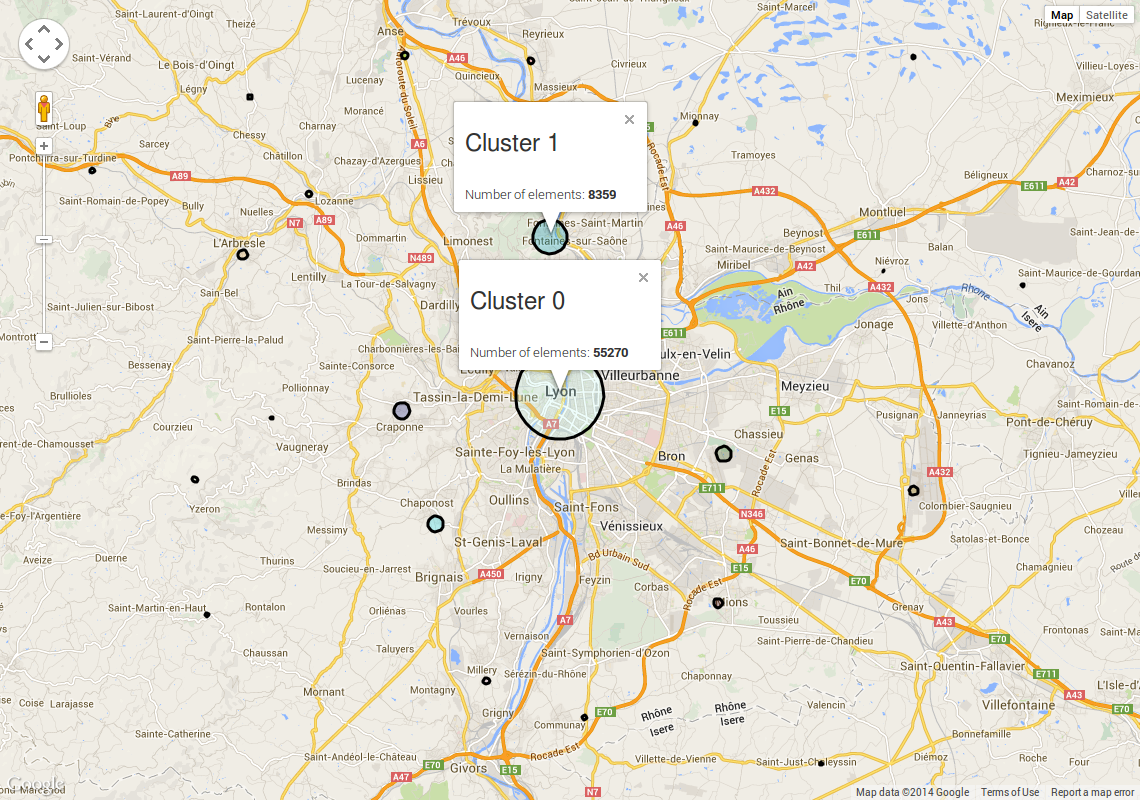
\includegraphics[width=16cm]{images/meanshift1.png}
    \caption{Meanshift, $q = 0.2$ et $n$ = 15}
    \label{fig:meanshift1}
\end{figure}

On remarque sans surprise qu'un cluster sort nettement du lot~: il s'agit du centre ville de Lyon, endroit où les photos Flickr sont les plus concentrées. Ce cluster comporte \textbf{55~270} photos, soit 69~\% des photos prises.

Le deuxième cluster est loin derrière, avec \textbf{8359} photos (soit 10.5~\% des photos prises), mais il reste néanmoins intéressant de constater que son centre se trouve exactement à \textit{La Demeure du Chaos} (Musée l'Organe). Il s'agit d'un ancien relais de poste qui a été transformé en musée d'art contemporain. Cela explique donc la présence d'un grand nombre de clichés à cet endroit (photos touristiques lors de la visite du musée).

Le paramétrage choisi ici est encore grossier. Il ne nous permet que de détecter les clusters sur de grandes étendues. Par exemple, nous ne pouvons pas nous contenter de ce paramétrage pour tenter de découvrir les différentes zones touristiques de Lyon (un seul cluster a été généré pour la ville de Lyon toute entière). Il nous faut pour cela diminuer le quantile.

La figure \vref{fig:meanshift2} tente d'illustrer les zones touristiques de Lyon en diminuant le quantile et en affichant également les points en plus des centres des clusters (la couleur choisie pour les points est celle de leur cluster d'appartenance).

\begin{figure}[!h]
    \centering
    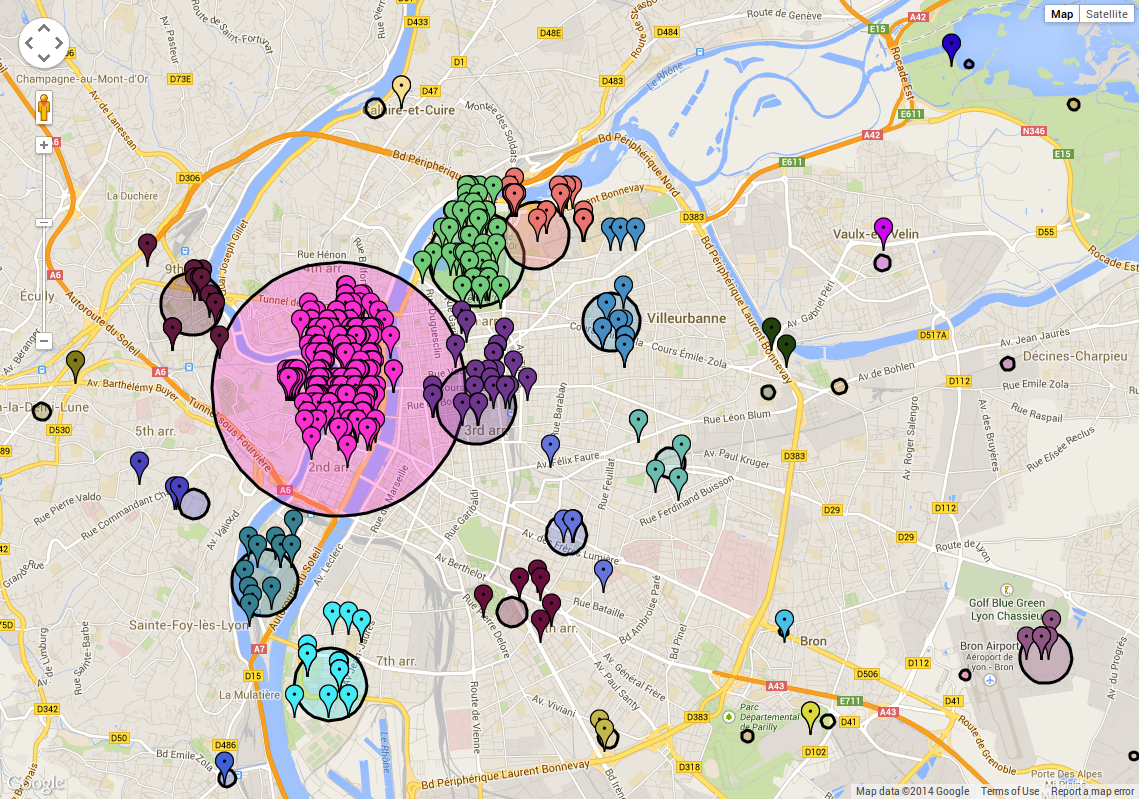
\includegraphics[width=16cm]{images/meanshift2.png}
    \caption{Meanshift, $q = 0.05$ et $n$ = 15}
    \label{fig:meanshift2}
\end{figure}

Cette représentation est déjà beaucoup plus intéressante. Le plus gros cluster (en rose-violet sur la figure \vref{fig:meanshift2}) est toujours situé au même endroit (centré entre la place Bellecour et l'Hôtel de Ville) et il représente le cœur touristique de Lyon.

On voit également apparaitre d'autres zones d'intérêt, comme le cluster vert, représentant avec certitude l'attrait des touristes pour le parc de la Tête d'Or, le cluster violet foncé, situé autour de la gare de la Part-Dieu, le cluster cyan représentant l'attrait pour le quartier de Gerland, ainsi que le \textit{Pôle de Commerces et de Loisirs de Confluence} (cluster vert foncé entre les deux fleuves), dont l'architecture très particulière incite à prendre des photos. On devine même le centre de ville de Villeurbanne (cluster bleu entre l'arrêt de métro République et Gratte Ciel).

Notons que si certains cercles (centres de clusters) n'ont aucun point à proximité, c'est parce que nous n'affichons qu'un pourcent de tous les points, alors que le calcul des clusters se fait lui sur l'ensemble de tous les points.

\newpage
\section{Kmeans}

Pour comparer nos résultats à ceux trouvés par d'autres méthodes de clustering, nous avons choisi d'utiliser la méthode de référence par excellence~: Kmeans.

Cette méthode est une bonne proposition alternative car~:
\begin{enumerate}

  \item elle est relativement "simple" à mettre en place, elle ne demande comme paramètres qu'un nombre de clusters à trouver et les données à partir desquelles les générer.
  \item c'est une méthode qui est utilisée par beaucoup de chercheurs pour comparer leurs résultats. Le fait que Kmeans soit familier de la plupart des chercheurs en data mining permet à ces personne de plus facilement détecter les performances demandées par le jeu de données présenté.
  \item c'est une méthode qui a quelques défauts, ce qui permet, par comparaison, de montrer l'intérêt de Meanshift.

\end{enumerate}
 
Nous avons donc essayé de reproduire avec Kmeans les mêmes conditions que les deux exemples avec Meanshift en lançant un Kmeans avec un nombre de clusters voulus à peu près équivalent à ceux trouvés ci-dessus.

\begin{figure}[!h]
    \centering
    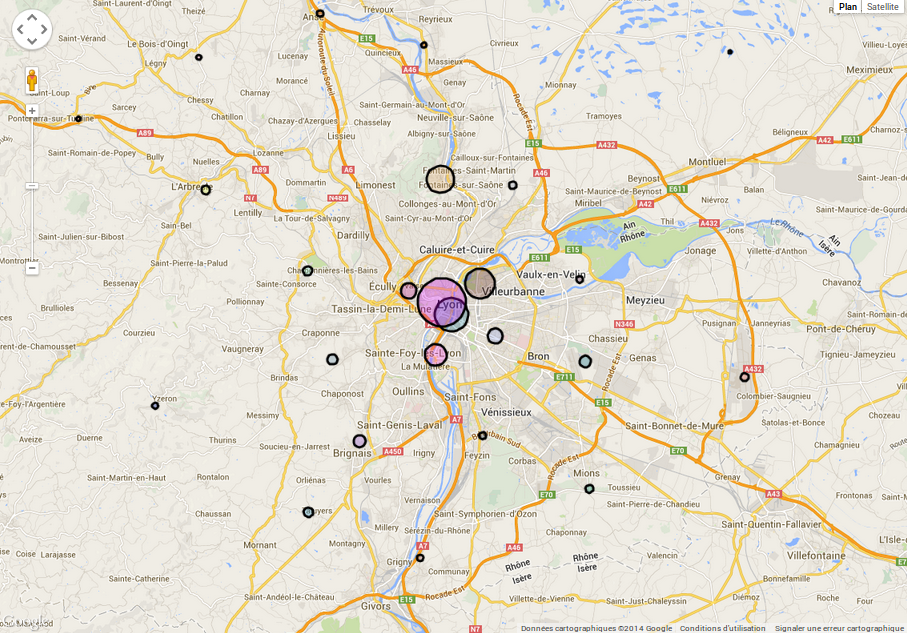
\includegraphics[width=16cm]{images/Kmeans1.png}
    \caption{K means, $nbClusters = 25$}
    \label{fig:Kmeans1}
\end{figure}

On remarque que Kmeans trouve, comme Meanshift, les petites villes dispersées autour de Lyon. Cependant il parvient à couper le centre ville en plus de clusters. Il semble avoir déjà repéré le parc de la Tête d'Or et commencé à différencier les quartiers de la Part-Dieu de la presqu'ile.
\\

\begin{figure}[!h]
    \centering
    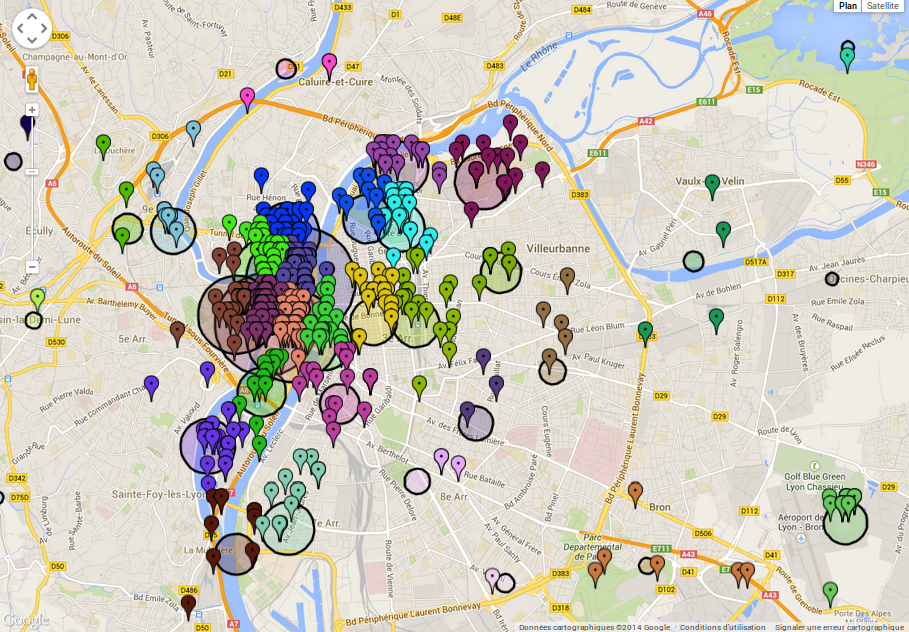
\includegraphics[width=16cm]{images/Kmeans2.png}
    \caption{K means, $nbClusters = 100$}
    \label{fig:Kmeans}
\end{figure}

Sur cette deuxième figure, Kmeans est dépassé en centre ville. Il découpe la presqu'ile et le parc de la tête d'or de manière on peut dire arbitraire sous la forme d'un damier.
Par contre les zones isolées comme l'aéroport de Lyon-Bron sont encore bien identifiées comme des clusters à part entière.
On peut en déduire que Kmeans devient inefficace dans des zones à trop forte densité de données tandis que Meanshift ne sert pas à grand chose sans un minimum de précision.
